% useful command to build & clean-up : 
% latexmk -pdf -outdir="French/Portfolio/PDF" -c "French/Portfolio/dossier_competences.tex"
% latexmk -pdf -outdir="French/Portfolio/PDF" "French/Portfolio/dossier_competences.tex"
% latexmk -c "French/Portfolio/dossier_competences.tex"
% find French/Portfolio/PDF -type f \( -name "*.aux" -o -name "*.log"  \) -delete


\documentclass{article}
\usepackage[scaled]{helvet}
\renewcommand{\familydefault}{\sfdefault} % applies font
\usepackage{tcolorbox}
\usepackage{xcolor}
\usepackage[export]{adjustbox} % for \raisebox

\usepackage[left=0.3in, right=0.3in, top=1.0in, bottom=1.0in]{geometry}
\usepackage{graphicx}
\usepackage{tikz}
\usepackage{hyperref}
\usepackage{enumitem}
\usepackage{fancyhdr}
\usepackage{titlesec}
\usepackage{microtype}
\usepackage{colortbl}
\usepackage{array} % Required for m{...} column type

% Define your own custom commands, styles, or formatting here

\pagestyle{fancy}
\fancyhf{}
\rhead{Alfred LALANNE}
\lhead{Dossier de compétences}
\cfoot{\thepage}

\title{Dossier de compétences}
\author{Alfred LALANNE}
\date{} % Remove the date

% Redefine \maketitle to remove the date and include photo
\makeatletter
\renewcommand{\maketitle}{%
    \begin{center} % Center the whole content
        \centering
        
        {\Large\bfseries \@title \par}
        \vskip 0.5em%
        {\large \@author \par}
        \begin{minipage}[b]{0.6\linewidth} % left minipage
            
        \end{minipage}%
        \hfill % Add some horizontal space between the minipages
        \begin{minipage}[b]{0.3\linewidth}   % right minipage
            \raggedleft
            \vspace*{-4\baselineskip} % Adjust the vertical position of the image
            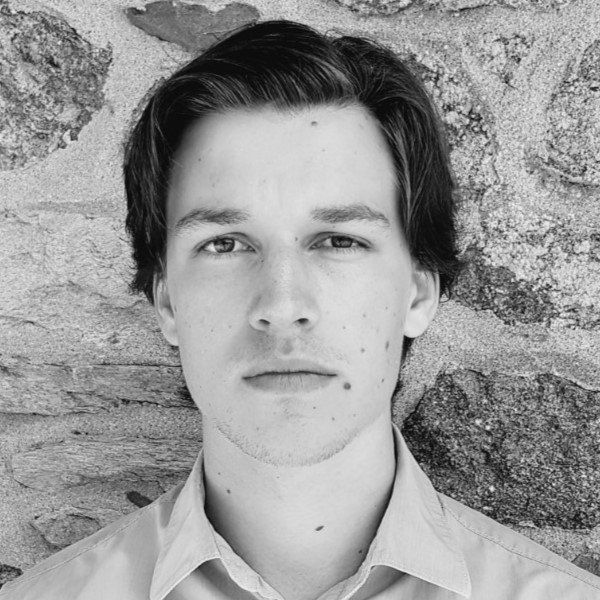
\includegraphics[width=0.7\linewidth]{moi.jpeg}
        \end{minipage}%
    \end{center} % End of center environment
}
\makeatother




\begin{document}

\maketitle

%\section{Domaines de compétence}

\definecolor{skyblue}{RGB}{135,206,235} % Define sky blue color

\definecolor{deepBlue}{RGB}{80,100,255} % Define deepBlue color
\definecolor{cream}{RGB}{255,253,208}
\definecolor{darkGray}{RGB}{64,64,64}
\definecolor{deepPurple}{RGB}{121, 53, 149}
\definecolor{enseaRed}{RGB}{191, 0, 80}


\begin{center}
    \begin{tikzpicture}
        \draw[enseaRed, line width=4pt] (-0.4\linewidth,-2pt) -- (0.4\linewidth,-2pt);
    \end{tikzpicture}
\end{center}

\begin{tabular}{@{}m{0.03\textwidth}@{\hspace{0.07\textwidth}}!{\color{deepPurple}\vline width 2pt}@{\hspace{0.025\textwidth}}m{0.75\textwidth}@{}}
    \textcolor{gray!80}{\raggedright Domaines\\ de\\ compétences} & % Use a subtle shade of blue
    \begin{itemize}[label={}, leftmargin=2em, topsep=0pt, partopsep=0pt, itemsep=0pt, parsep=0pt] % Remove bullet points and adjust left margin
        \setlength{\itemsep}{0pt} % Reduce spacing between lines

        \item \textcolor{gray!150}{Hardware - Electronique}
        \begin{itemize}[label={\textcolor{gray!80}{--}}, leftmargin=2em, topsep=0pt, partopsep=0pt, itemsep=0pt, parsep=0pt] % reduce spacing & adjust left margin
            \item \textcolor{gray!80}{Conception de schémas électriques, routage, simulation }
            \item \textcolor{gray!80}{Filtrage analogique actif et passif, Matlab}
        \end{itemize}

        \item \textcolor{gray!150}{Electronique numérique} 
        \begin{itemize}[label={\textcolor{gray!80}{--}}, leftmargin=2em, topsep=0pt, partopsep=0pt, itemsep=0pt, parsep=0pt] % reduce spacing & adjust left margin
            \item \textcolor{gray!80}{Microcontrôleurs : programmation en C et Assembleur sur Keil-uVision }
            \item \textcolor{gray!80}{Logique programmable : technologie FPGA, description VHDL}
            \item \textcolor{gray!80}{Systèmes sur puce : SoC, SoC-FPGA, SoC-IP}
        \end{itemize}

        \item \textcolor{gray!150}{Informatique}
        \begin{itemize}[label={\textcolor{gray!80}{--}}, leftmargin=2em, topsep=0pt, partopsep=0pt, itemsep=0pt, parsep=0pt] % reduce spacing & adjust left margin
            \item \textcolor{gray!80}{Programmation bas-niveau : microcontrôleurs, FreeRTOS}
            \item \textcolor{gray!80}{Traitement d'image}
            \item \textcolor{gray!80}{Développement jeux-vidéos}
        \end{itemize}

        \item \textcolor{gray!150}{Ingénierie système}
        \begin{itemize}[label={\textcolor{gray!80}{--}}, leftmargin=2em, topsep=0pt, partopsep=0pt, itemsep=0pt, parsep=0pt] % reduce spacing & adjust left margin
            \item \textcolor{gray!80}{Rédaction de cahier des charges}
            \item \textcolor{gray!80}{Etudes de faisabilité}
        \end{itemize}
    \end{itemize}
\end{tabular}


%%%%%%%%%%%%%%%%%%%%%%%%%%%%%%%%%%%%%%%%%%%%%%%%%%%%%%%%%%%%%%%%%%%%%%%%%%%%%%%%%%%%%%%%%%%%%%%%%%%%%%%%%%%%%%%%%%%%%%%%%%%%%%%%%%%%%%%%%%%%%%%%%%%%

\begin{center}
    \begin{tikzpicture}
        \draw[enseaRed, line width=4pt] (-0.4\linewidth,-2pt) -- (0.4\linewidth,-2pt);
    \end{tikzpicture}
\end{center}


\begin{tabular}{@{}m{0.03\textwidth}@{\hspace{0.07\textwidth}}!{\color{deepPurple}\vline width 2pt}@{\hspace{0.025\textwidth}}m{0.75\textwidth}@{}}
    \textcolor{gray!80}{Langages\newline Outils\newline Normes} & 
    \begin{itemize}[label={}, leftmargin=2em, topsep=0pt, partopsep=0pt, itemsep=0pt, parsep=0pt] 
        \setlength{\itemsep}{0pt} % Reduce spacing between lines

        \item \textcolor{gray!150}{Langages}
        \begin{itemize}[label={\textcolor{gray!80}{}}, leftmargin=2em, topsep=0pt, partopsep=0pt, itemsep=0pt, parsep=0pt] 
            \item \textcolor{gray!80}{C, C++, Python, Java, Assembleur}
        \end{itemize}

        \item \textcolor{gray!150}{Outils}
        \begin{itemize}[label={\textcolor{gray!80}{--}}, leftmargin=2em, topsep=0pt, partopsep=0pt, itemsep=0pt, parsep=0pt] % reduce spacing & adjust left margin
            \item \textcolor{gray!80}{Collaboratifs : Git, Jira, Confluence, Teams}
            \item \textcolor{gray!80}{IDEs : VSCode, STM32CubeIDE, Eclipse}
            \item \textcolor{gray!80}{Bibliothèques : OpenCV, PyQt5, NumPy, SFML, Matplotlib, RealSense}
            \item \textcolor{gray!80}{Modélisation : OrCAD PSpice, Visio, Blender, draw.io}
        \end{itemize}

        \item \textcolor{gray!150}{Normes}
        \begin{itemize}[label={\textcolor{gray!80}{}}, leftmargin=2em, topsep=0pt, partopsep=0pt, itemsep=0pt, parsep=0pt] 
            \item \textcolor{gray!80}{ISO7816, ISO12233}
        \end{itemize}
    \end{itemize}
\end{tabular}


%%%%%%%%%%%%%%%%%%%%%%%%%%%%%%%%%%%%%%%%%%%%%%%%%%%%%%%%%%%%%%%%%%%%%%%%%%%%%%%%%%%%%%%%%%%%%%%%%%%%%%%%%%%%%%%%%%%%%%%%%%%%%%%%%%%%%%%%%%%%%%%%%%%%

\begin{center}
    \begin{tikzpicture}
        \draw[enseaRed, line width=4pt] (-0.4\linewidth,-2pt) -- (0.4\linewidth,-2pt);
    \end{tikzpicture}
\end{center}


\begin{tabular}{@{}m{0.03\textwidth}@{\hspace{0.07\textwidth}}!{\color{deepPurple}\vline width 2pt}@{\hspace{0.025\textwidth}}m{0.75\textwidth}@{}}
    \textcolor{gray!80}{Secteurs d'activités} & 
    \textcolor{gray!80}{Systèmes d’identification et de sécurité} \newline 
    \textcolor{gray!80}{Système d'acquisition automatisé} \newline 
\end{tabular}


%%%%%%%%%%%%%%%%%%%%%%%%%%%%%%%%%%%%%%%%%%%%%%%%%%%%%%%%%%%%%%%%%%%%%%%%%%%%%%%%%%%%%%%%%%%%%%%%%%%%%%%%%%%%%%%%%%%%%%%%%%%%%%%%%%%%%%%%%%%%%%%%%%%%

\begin{center}
    \begin{tikzpicture}
        \draw[enseaRed, line width=4pt] (-0.4\linewidth,-2pt) -- (0.4\linewidth,-2pt);
    \end{tikzpicture}
\end{center}


\begin{tabular}{@{}m{0.03\textwidth}@{\hspace{0.07\textwidth}}!{\color{deepPurple}\vline width 2pt}@{\hspace{0.025\textwidth}}m{0.65\textwidth}@{}m{0.6\linewidth}@{}}
    \textcolor{gray!80}{Formation} & 
    \textcolor{gray!150}{Ingénieur électronicien ENSEA}
    \begin{itemize}[label={\textcolor{gray!80}{--}}, leftmargin=2em, topsep=0pt, partopsep=0pt, itemsep=0pt, parsep=0pt] % reduce spacing & adjust left margin
        \item \textcolor{gray!80}{Année d'obtention du diplôme : 2023}
        \item \textcolor{gray!80}{Spécialités : microélectronique et numérique} 
    \end{itemize} &
    \raisebox{4\height}{
\includegraphics[width=0.1\linewidth,valign=t]{ensea.jpg}} % adjust the raisebox value as needed
\end{tabular}


%%%%%%%%%%%%%%%%%%%%%%%%%%%%%%%%%%%%%%%%%%%%%%%%%%%%%%%%%%%%%%%%%%%%%%%%%%%%%%%%%%%%%%%%%%%%%%%%%%%%%%%%%%%%%%%%%%%%%%%%%%%%%%%%%%%%%%%%%%%%%%%%%%%%





\end{document}